\documentclass[11pt,a4paper]{article}

\usepackage[T1]{fontenc}
\usepackage[utf8]{inputenc}
\usepackage[brazilian]{babel}
\usepackage{amsmath, amssymb}
\usepackage{booktabs}
\usepackage{graphicx}
\usepackage{float}
\usepackage[margin=2.5cm]{geometry}
\usepackage{microtype}
\usepackage{xcolor}
\usepackage[hidelinks]{hyperref}
\usepackage{setspace}
\onehalfspacing
\graphicspath{{figuras_sem_motos/}}

\newcommand{\reais}[1]{R\$\,#1}

\title{\textbf{Valor monetário do patrimônio recuperado pela Força Municipal}\\[0.3em]
\large Um modelo probabilístico com distribuição de modelos e preços de mercado\\(Rio de Janeiro, março--junho de 2026)}
\author{Prefeitura do Rio --- Secretaria Municipal de Desenvolvimento Econômico \& COMPSTAT RIO}
\date{\today}

\begin{document}
\maketitle

\begin{abstract}
\noindent Estimamos o valor monetário do patrimônio recuperado pela Força Municipal
(SEGUR/Prefeitura do Rio) entre 15 de março e 8 de junho de 2026: 118 celulares, 19 bicicletas e
15 cordões. Tratamos o valor de cada item recuperado como uma \emph{variável aleatória}:
sorteia-se o modelo segundo a distribuição real do que é roubado na cidade (ponderada por
frequência) e o preço a partir de uma amostra de preços de mercado, em duas bases ---
\textbf{revenda} (usado) e \textbf{reposição} (novo). Agregando por simulação de Monte Carlo, o
valor esperado do conjunto é de \textbf{\reais{163} mil} a preços de revenda (banda de 90\%:
\reais{145}--\reais{181} mil) e \textbf{\reais{267} mil} a preços de reposição
(\reais{237}--\reais{299} mil); o envelope extremo vai de \reais{44} mil a \reais{1{,}24} milhão.
Os celulares concentram cerca de 88\% do valor. Todas as cifras têm fonte pública (coleta em
16/06/2026).
\end{abstract}

% =====================================================================
\section{Introdução}
% =====================================================================
Entre 15 de março e 8 de junho de 2026, a Força Municipal (Secretaria Especial de Segurança
Urbana --- SEGUR, Prefeitura do Rio de Janeiro) reportou a recuperação de 118 celulares, 19
bicicletas e 15 cordões. Quanto vale, em reais, esse patrimônio?

A resposta não é um número único. Um celular recuperado pode ser um aparelho de entrada usado de
algumas centenas de reais ou um \emph{flagship} novo de mais de dez mil; um cordão pode ser uma
semijoia folheada ou uma peça de ouro. Responder ``quanto vale'' exige, então, estimar a
\emph{distribuição} de valores plausíveis --- a probabilidade de que um item recuperado valha
cada quantia --- e não apenas uma média.

A contribuição desta nota é tratar o valor recuperado como uma variável aleatória, cuja
distribuição é construída a partir (i) da composição real do que é roubado na cidade e (ii) de
preços de mercado coletados por modelo, nas bases de revenda (usado) e de reposição (novo). Por
\emph{revenda} entende-se a compra do bem \emph{usado} (quanto ele valeria se revendido); por
\emph{reposição}, a compra do equivalente \emph{novo} (o custo de repô-lo). Isso
produz, para cada categoria, uma distribuição de probabilidade de valor, e, para o conjunto, uma
estimativa com intervalo de confiança --- tudo referenciado a fontes públicas.

% =====================================================================
\section{Metodologia}
% =====================================================================

\subsection{Modelo probabilístico}
Seja $i$ uma categoria de item ($\text{cel}$, $\text{bike}$, $\text{cord}$) e
$b\in\{\text{rev},\text{rep}\}$ a base de valor (revenda ou reposição). O valor de uma unidade
recuperada da categoria $i$ é a variável aleatória de \textbf{mistura}
\begin{equation}
  V_i^{\,b}\;\sim\;\sum_{m\in\mathcal{M}_i} w_{i,m}\,\hat F_{i,m}^{\,b},
  \label{eq:mix}
\end{equation}
em que $\mathcal{M}_i$ é o conjunto de modelos representativos, $w_{i,m}$ é o peso do modelo $m$
($\sum_m w_{i,m}=1$) e $\hat F_{i,m}^{\,b}$ é a distribuição empírica dos preços coletados para o
modelo $m$ na base $b$. Sorteia-se um modelo segundo os pesos e, em seguida, um preço a partir das
observações daquele modelo. Seu valor esperado e variância são
\begin{equation}
  \mathbb{E}[V_i^{b}]=\sum_m w_{i,m}\,\bar p_{i,m}^{\,b},
  \qquad
  \mathrm{Var}(V_i^{b})=\sum_m w_{i,m}\Big(\sigma_{i,m}^{b\,2}+\big(\bar p_{i,m}^{b}-\mathbb{E}[V_i^b]\big)^2\Big).
  \label{eq:moments}
\end{equation}
O valor total recuperado é a soma sobre todas as unidades:
\begin{equation}
  V^{\,b}=\sum_{i}\sum_{k=1}^{N_i} V_{i,k}^{\,b},
  \qquad
  \mathbb{E}[V^{b}]=\sum_i N_i\,\mathbb{E}[V_i^{b}],
  \qquad
  \mathrm{Var}(V^{b})=\sum_i N_i\,\mathrm{Var}(V_i^{b}),
  \label{eq:total}
\end{equation}
com $N_i$ a quantidade recuperada (painel da SEGUR). Nenhum ``fator de depreciação'' arbitrário é
aplicado: a base de revenda já é preço de usado (o mercado precifica o desgaste) e a de reposição
é o preço de novo.

\subsection{Distribuição de modelos por frequência}
Os pesos $w_{i,m}$ vêm de \emph{fontes de frequência}, pois o item recuperado é o que se rouba na
rua. Para celulares, a participação por marca é a do roubo (Anuário do Fórum Brasileiro de
Segurança Pública: Samsung 37\%, Apple 25\%, Motorola 23\%, Xiaomi 10\%), ajustada pelo perfil
socioeconômico (TIC Domicílios) em direção a modelos de entrada/intermediário. As bicicletas
refletem o que \emph{pessoas físicas} compram e têm furtado --- bicicletas de varejo popular
(Caloi/Mormaii) e usados do Rio (OLX-RJ, Caloi $\approx$70\%). Os cordões seguem a prevalência de
folheado vs.\ ouro.

\subsection{Coleta de preços e distribuições empíricas}
Para cada modelo coletou-se uma \textbf{amostra de preços observados} (16/06/2026): 289
observações entre usado e novo. As fontes de usado incluem o varejo de seminovos
(Trocafy/Trocafone, cada listagem = um preço) e anúncios do Rio (OLX-RJ); as de novo, o varejo
(Magazine Luiza, Samsung, Apple, Caloi/Mormaii) e joalherias por gramatura (cordões = peso
$\times$ cotação do ouro 18k). OLX e Mercado Livre, que bloqueiam acesso automatizado, entraram
apenas por trechos de busca. Cada amostra é, portanto, uma aproximação (não um censo); os tamanhos
por modelo estão em \texttt{dados\_distribuicao.json}.

\subsection{Agregação por Monte Carlo}\label{sec:mc}
A distribuição de $V_i^b$ e de $V^b$ é obtida por simulação: sorteiam-se $N_i$ unidades por
categoria segundo a Eq.~\eqref{eq:mix}, somam-se, e repete-se 50.000 vezes (semente fixa, para
reprodutibilidade). Reporta-se o valor esperado e a banda de 90\% (percentis 5 e 95).

\subsection{Caso especial: distribuição dos cordões}
Os cordões merecem tratamento à parte. O que é arrancado na rua é, na maioria,
\textbf{folheado/semijoia} (\reais{15}--\reais{150}) ou ouro \emph{leve} (2--8\,g) --- raramente
peças pesadas de joalheria. A distribuição é, portanto, \textbf{fortemente assimétrica à direita}
(\emph{lognormal-like}): mediana no folheado (\reais{50}--\reais{80}) e média puxada por uma cauda
longa e fina de ouro. Calibramos a amostra para $\approx$80\% folheado/baixo valor, $\approx$18\%
ouro leve e $\approx$2--4\% de cauda (eventos raros, tipicamente golpes dirigidos, não o arranco de
rua), com teto realista contido (\reais{3.000} usado / \reais{5.000} novo). Dois fatos sustentam a
forma: o mercado de semijoias é massivo e popular (``luxo acessível''), e o canal de receptação
realiza só $\approx$50--65\% do valor --- comprimindo ainda mais a base. Daí o desvio $\gg$ média
na Tabela~\ref{tab:itens}, assinatura da assimetria. Fontes: IBGM (mercado de semijoias); preços de
folheado (Shekinah; Prata Pura); ouro leve de uso diário 1,8--8\,g (Dr Joias; Pyter); cotação do
ouro 18k $\approx$\reais{530}/g; e o caso de Linhares-ES (cordão ``de R\$\,200 mil'' revendido por
R\$\,104 mil) ilustrando a cauda rara.

% =====================================================================
\section{Resultados}
% =====================================================================

\subsection{Distribuição de valor por item}
A Figura~\ref{fig:itens} mostra a distribuição de valor de uma unidade recuperada de cada
categoria, nas duas bases. As formas são informativas: o celular é fortemente assimétrico à
direita (massa em aparelhos de entrada, cauda nos \emph{flagships}); o cordão é praticamente
bimodal (folheados de baixo valor e peças de ouro). A Tabela~\ref{tab:itens} resume os momentos.

\begin{figure}[H]
  \centering
  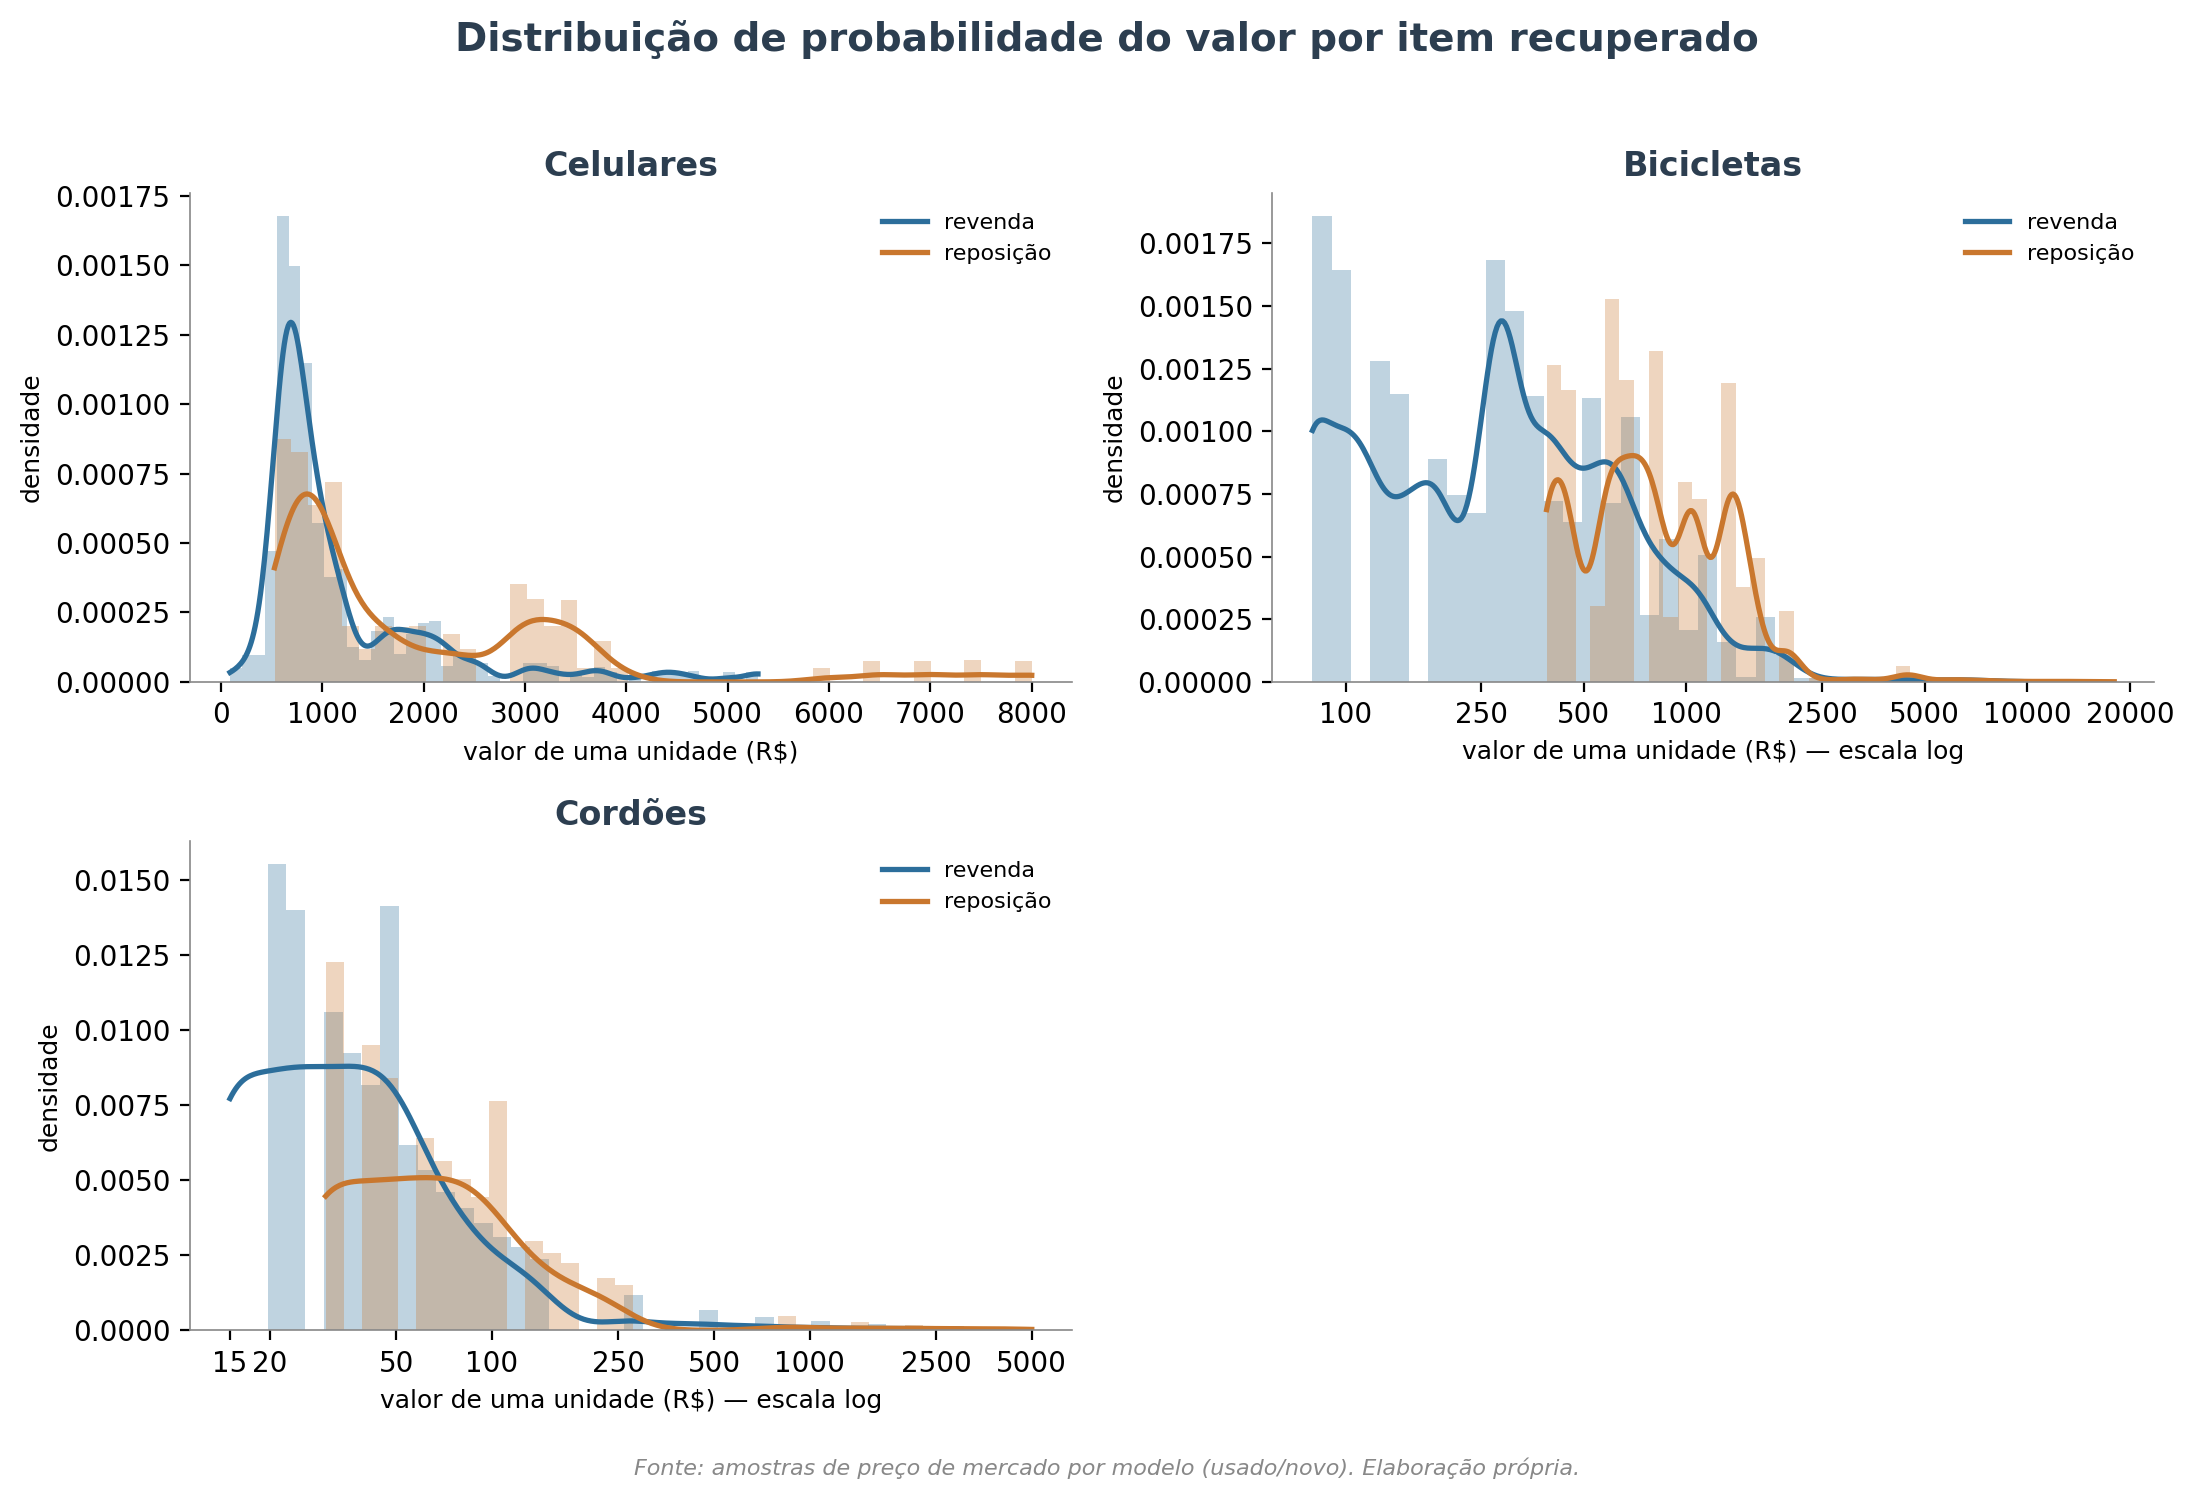
\includegraphics[width=\linewidth]{dist_itens}
  \caption{Distribuição de probabilidade do valor de uma unidade recuperada, por categoria
  (azul: revenda/usado; laranja: reposição/novo). Histograma das amostras com densidade KDE.}
  \label{fig:itens}
\end{figure}

\begin{table}[H]
  \centering\small
  \begin{tabular}{llrrr}
    \toprule
    Item & base & $\mathbb{E}[V_i]$ & desvio & faixa p5--p95 \\
    \midrule
    Celulares  & revenda   & 1.212 & 944   & 530--3.500 \\
               & reposição & 1.964 & 1.641 & 619--6.500 \\
    Bicicletas & revenda   & 668   & 472   & 120--1.800 \\
               & reposição & 1.115 & 684   & 410--2.000 \\
    Cordões    & revenda   & 462   & 804   & 20--2.400 \\
               & reposição & 936   & 1.486 & 40--5.000 \\
    \bottomrule
  \end{tabular}
  \caption{Momentos da distribuição de valor por unidade (R\$), por base. Fonte: amostras de
  preço de mercado; simulação de Monte Carlo.}
  \label{tab:itens}
\end{table}

\subsection{Valor total recuperado}
Agregando (Eq.~\eqref{eq:total}), o valor esperado do patrimônio recuperado é de
\textbf{\reais{186} mil} a preços de revenda e \textbf{\reais{312} mil} a preços de reposição. A
Figura~\ref{fig:total} mostra as duas distribuições com suas bandas de 90\%
(\reais{163}--\reais{211} mil e \reais{271}--\reais{357} mil). A Tabela~\ref{tab:contrib} detalha a
contribuição por categoria: os \textbf{celulares} respondem por cerca de \textbf{88\%} do total.

\begin{figure}[H]
  \centering
  
\includegraphics[width=0.92\linewidth]{dist_total}
  \caption{Distribuição do valor total recuperado por simulação de Monte Carlo (50.000 iterações);
  linha = valor esperado, faixa sombreada = banda de 90\%.}
  \label{fig:total}
\end{figure}

\begin{table}[H]
  \centering\small
  \begin{tabular}{lrrrr}
    \toprule
    Item & $N_i$ & Contrib.\ revenda & Contrib.\ reposição & \% (revenda) \\
    \midrule
    Celulares  & 118 & 143.016 & 231.752 & 87,9\% \\
    Bicicletas & 19  & 12.692  & 21.185  & 7,8\% \\
    Cordões    & 15  & 6.930   & 14.040  & 4,3\% \\
    \midrule
    \textbf{Total} & — & \textbf{$\approx$162.638} & \textbf{$\approx$266.977} & 100\% \\
    \bottomrule
  \end{tabular}
  \caption{Contribuição por categoria ($N_i\cdot\mathbb{E}[V_i]$) e total (R\$).}
  \label{tab:contrib}
\end{table}

\noindent A banda de 90\% reflete a incerteza de \emph{amostragem} do total. A incerteza
\emph{estrutural} é capturada pela distância entre as bases de revenda e reposição
(\reais{163}--\reais{267} mil) e pelo \textbf{envelope extremo} de \reais{44} mil (se cada item
fosse o modelo usado mais barato) a \reais{1{,}24} milhão (se cada item fosse o modelo novo mais
caro).

% =====================================================================
\section{Conclusões}
% =====================================================================
O patrimônio recuperado pela Força Municipal no período vale, em valor esperado, entre \reais{163}
mil (revenda) e \reais{267} mil (reposição), com envelope de \reais{44} mil a \reais{1{,}24}
milhão. O resultado é dominado pelos celulares ($\approx$88\%). O tratamento probabilístico mostra
não só um número, mas a \emph{distribuição} de valores plausíveis de cada item, ancorada na
composição real do que se rouba na cidade e em preços de mercado verificáveis. A atualização para
janelas futuras entra apenas trocando os $N_i$.

% =====================================================================
\section*{Limitações}
% =====================================================================
\begin{itemize}\setlength\itemsep{0.1em}
  \item \textbf{Distribuição é proxy:} o \emph{mix} exato dos itens recuperados não foi divulgado;
        os pesos vêm da frequência de roubo/vendas, e a maioria das cifras é nacional, não recorte
        do Rio.
  \item \textbf{Amostras de preço, não censo:} OLX e Mercado Livre bloqueiam coleta automatizada;
        usaram-se varejo de seminovos, anúncios e joalherias.
  \item \textbf{Bicicletas:} avaliadas como bens de uso pessoal (compradas por pessoas físicas),
        que são as efetivamente furtadas; bicicletas de sistema compartilhado não entram na conta.
\end{itemize}

% =====================================================================
\section*{Fontes}
% =====================================================================
\small
\noindent Coleta em 16/06/2026. Inventário (formato F-T.N) em \texttt{inventario\_fontes.md};
amostras de preço por modelo (com $n$ e URL) em \texttt{dados\_distribuicao.json}.
(FÓRUM BRAS.\ DE SEGURANÇA PÚBLICA. ``Marcas de celulares mais roubadas'', via Exame/InfoMoney, 2024) ·
(STATCOUNTER. ``Mobile Vendor Share Brazil'', 2026) ·
(CETIC.BR. ``TIC Domicílios'', 2024) ·
(TROCAFY/TROCAFONE. ``Seminovos por listagem'', 2026) ·
(MAGAZINE LUIZA; SAMSUNG; APPLE; CALOI. ``Preços de varejo (novo)'', 2026) ·
(OLX. ``Bicicletas e celulares usados, RJ'', 2024--2026) ·
(OURO RIO DE JANEIRO. ``Cotação do ouro 18k'', 2026) ·
(RDJ JOIAS; VITALE JOIAS. ``Cordões ouro 18k e folheados'', 2026).

\end{document}
